%%%%%%%%%%%%%%%%%%%%%%%%%%%%%%%%%%%%%%%%%
% University/School Laboratory Report
% LaTeX Template
% Version 3.1 (25/3/14)
%
% This template has been downloaded from:
% http://www.LaTeXTemplates.com
%
% Original author:
% Linux and Unix Users Group at Virginia Tech Wiki
% (https://vtluug.org/wiki/Example_LaTeX_chem_lab_report)
%
% License:
% CC BY-NC-SA 3.0 (http://creativecommons.org/licenses/by-nc-sa/3.0/)
%
%%%%%%%%%%%%%%%%%%%%%%%%%%%%%%%%%%%%%%%%%

%----------------------------------------------------------------------------------------
%	PACKAGES AND DOCUMENT CONFIGURATIONS
%----------------------------------------------------------------------------------------

\documentclass{article}

\usepackage{graphicx} % Required for the inclusion of images
\usepackage{natbib} % Required to change bibliography style to APA
\usepackage{amsmath} % Required for some math elements
\usepackage{mathtools}
\usepackage[export]{adjustbox}
\usepackage{subcaption}
\usepackage{float}
\usepackage{listings}
\usepackage{minted}

\DeclarePairedDelimiter{\abs}{\lvert}{\rvert}
\setlength\parindent{0pt} % Removes all indentation from paragraphs

\renewcommand{\labelenumi}{\alph{enumi}.} % Make numbering in the enumerate environment by letter rather than number (e.g. section 6)

%\usepackage{times} % Uncomment to use the Times New Roman font

%----------------------------------------------------------------------------------------
%	DOCUMENT INFORMATION
%----------------------------------------------------------------------------------------

\title{ECE 637 Digital Image Processing Laboratory: \\ Neighborhoods and Connected Components} % Title

\author{Yang \textsc{Wang}} % Author name

\date{\today} % Date for the report

\begin{document}

\maketitle % Insert the title, author and date

% If you wish to include an abstract, uncomment the lines below
% \begin{abstract}
% Abstract text
% \end{abstract}

% If you have more than one objective, uncomment the below:
%\begin{description}
%\item[First Objective] \hfill \\
%Objective 1 text
%\item[Second Objective] \hfill \\
%Objective 2 text
%\end{description}

%\subsection{Definitions}
%\label{definitions}
%\begin{description}
%\item[Stoichiometry]
%The relationship between the relative quantities of substances taking part in a reaction or forming a compound, typically a ratio of whole integers.
%\item[Atomic mass]
%The mass of an atom of a chemical element expressed in atomic mass units. It is approximately equivalent to the number of protons and neutrons in the atom (the mass number) or to the average number allowing for the relative abundances of different isotopes.
%\end{description}

%----------------------------------------------------------------------------------------
%	SECTION 1
%----------------------------------------------------------------------------------------

\section{Area Fill}
	In this section, a C program that fills in an area of connected pixels in a
	image is written. C subroutine to find the connected neighbors of a specfic
	pixel and to find all the pixels connected to a specfic pixel is implemented.

\subsection{Plot image im22gd2.tif}
	\begin{figure}[h]
		\begin{center}
			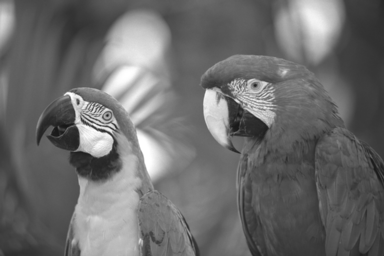
\includegraphics[width=0.8\textwidth]{img22gd2.png}
			\caption{Original img22gd2.tif}
		\end{center}
	\end{figure}

\pagebreak

\subsection{Plot image showing the connected set for $s=(67,45)$, and $T=2$}
	\begin{figure}[h]
		\begin{center}
			
\includegraphics[width=0.65\textwidth]{img22gd2_af2.png}
			\caption{$s=(67,45)$, and $T=2$}
		\end{center}
	\end{figure}

\subsection{Plot image showing the connected set for $s=(67,45)$, and $T=1$}
	As we can see, when $T$ gets smaller, there is less connected set.
	\begin{figure}[h]
		\begin{center}
			
\includegraphics[width=0.65\textwidth]{img22gd2_af1.png}
			\caption{$s=(67,45)$, and $T=1$}
		\end{center}
	\end{figure}

\pagebreak

\subsection{Plot image showing the connected set for $s=(67,45)$, and $T=3$}
	As we can see, when $T$ gets bigger, there are more connected sets.
	\begin{figure}[h]
		\begin{center}
			
\includegraphics[width=0.65\textwidth]{img22gd2_af3.png}
			\caption{$s=(67,45)$, and $T=3$}
		\end{center}
	\end{figure}

\subsection{Code listing}
	\subsubsection{areafill.c}
		\inputminted[tabsize=4,breaklines]{c}{areafill.c}
	\subsubsection{defs.c}
		Note: Section 2 uses the same subroutines written
		in this code listing.
		\inputminted[tabsize=4,breaklines]{c}{defs.c}
	\subsubsection{defs.h}
		\inputminted[tabsize=4,breaklines]{c}{defs.h}

\pagebreak

%----------------------------------------------------------------------------------------
%	SECTION 2
%----------------------------------------------------------------------------------------
\section{Image Segmentation}
	In this section, instead of using only one pixel to grow the connected
	sets, we index through the image to extract all the connected sets in
	the original image. Hence, an image segmentation is performed in this
	section.

\subsection{Plot image segmentation for $T=1$}
	\begin{figure}[h]
		\begin{center}
			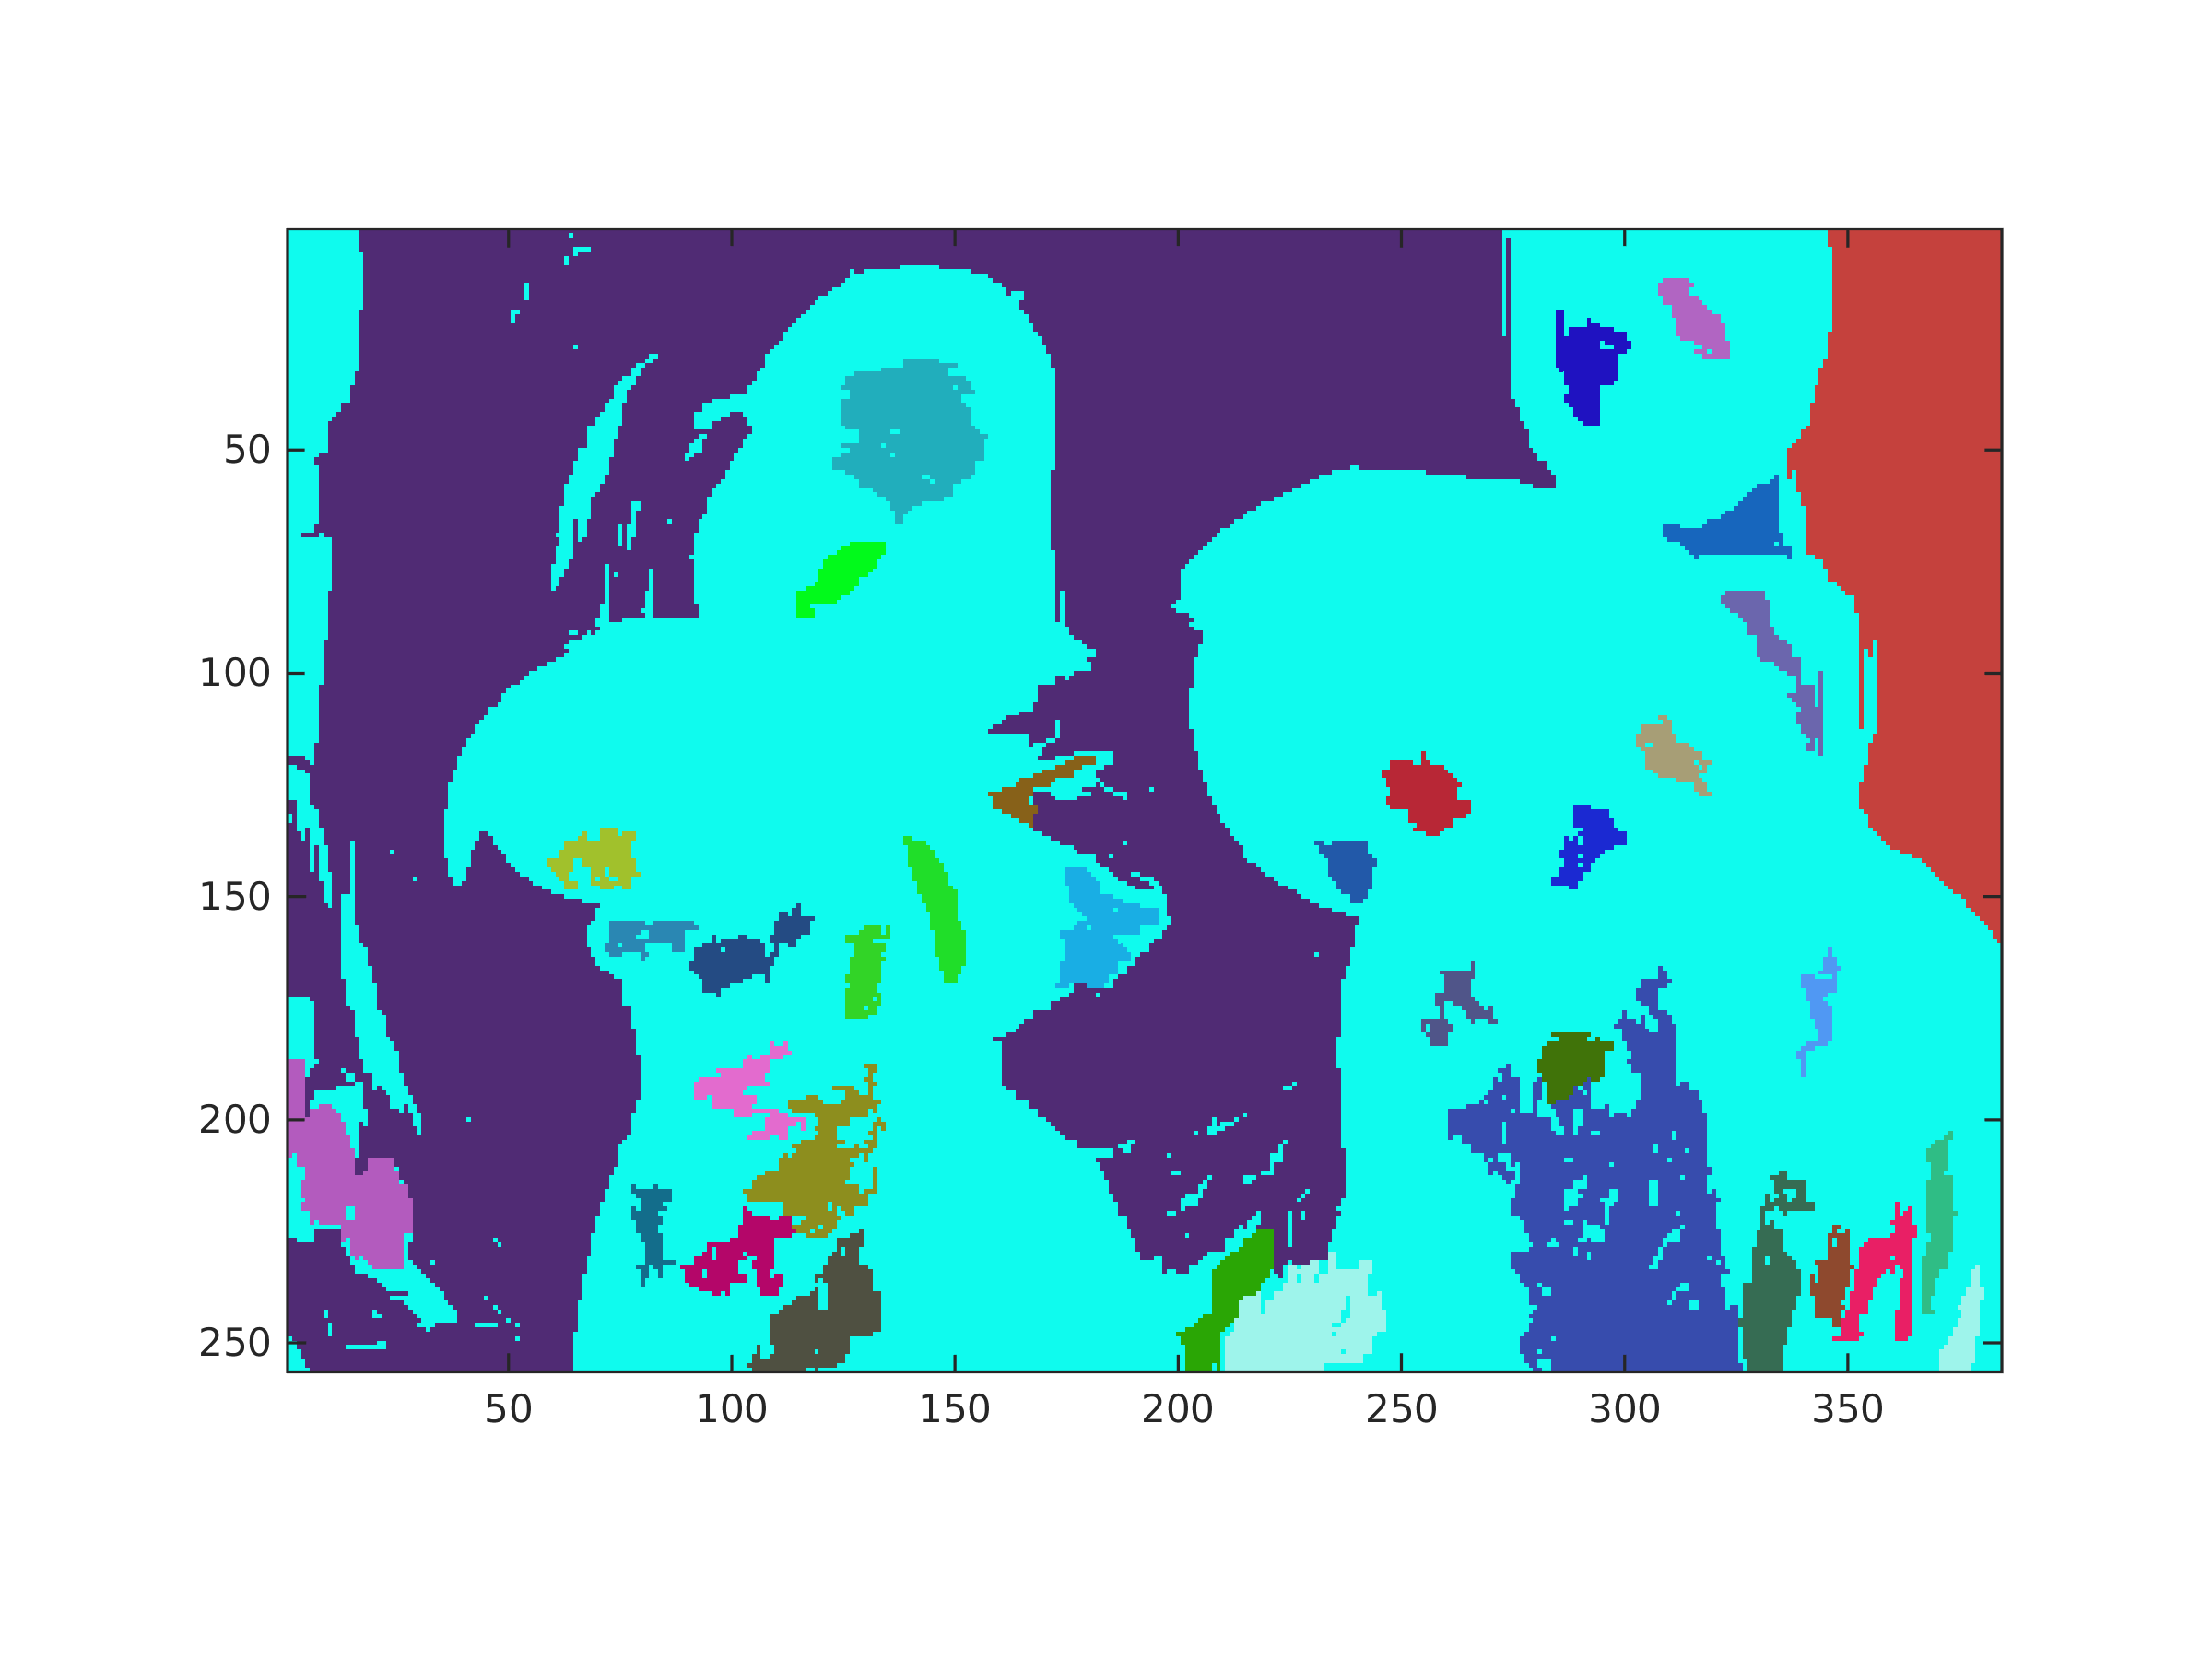
\includegraphics[width=0.65\textwidth]{img22gd2_sm1.png}
			\caption{Randomly colored segmentation for $T=1$}
		\end{center}
	\end{figure}

\subsection{Plot image segmentation for $T=2$}
	\begin{figure}[h]
		\begin{center}
			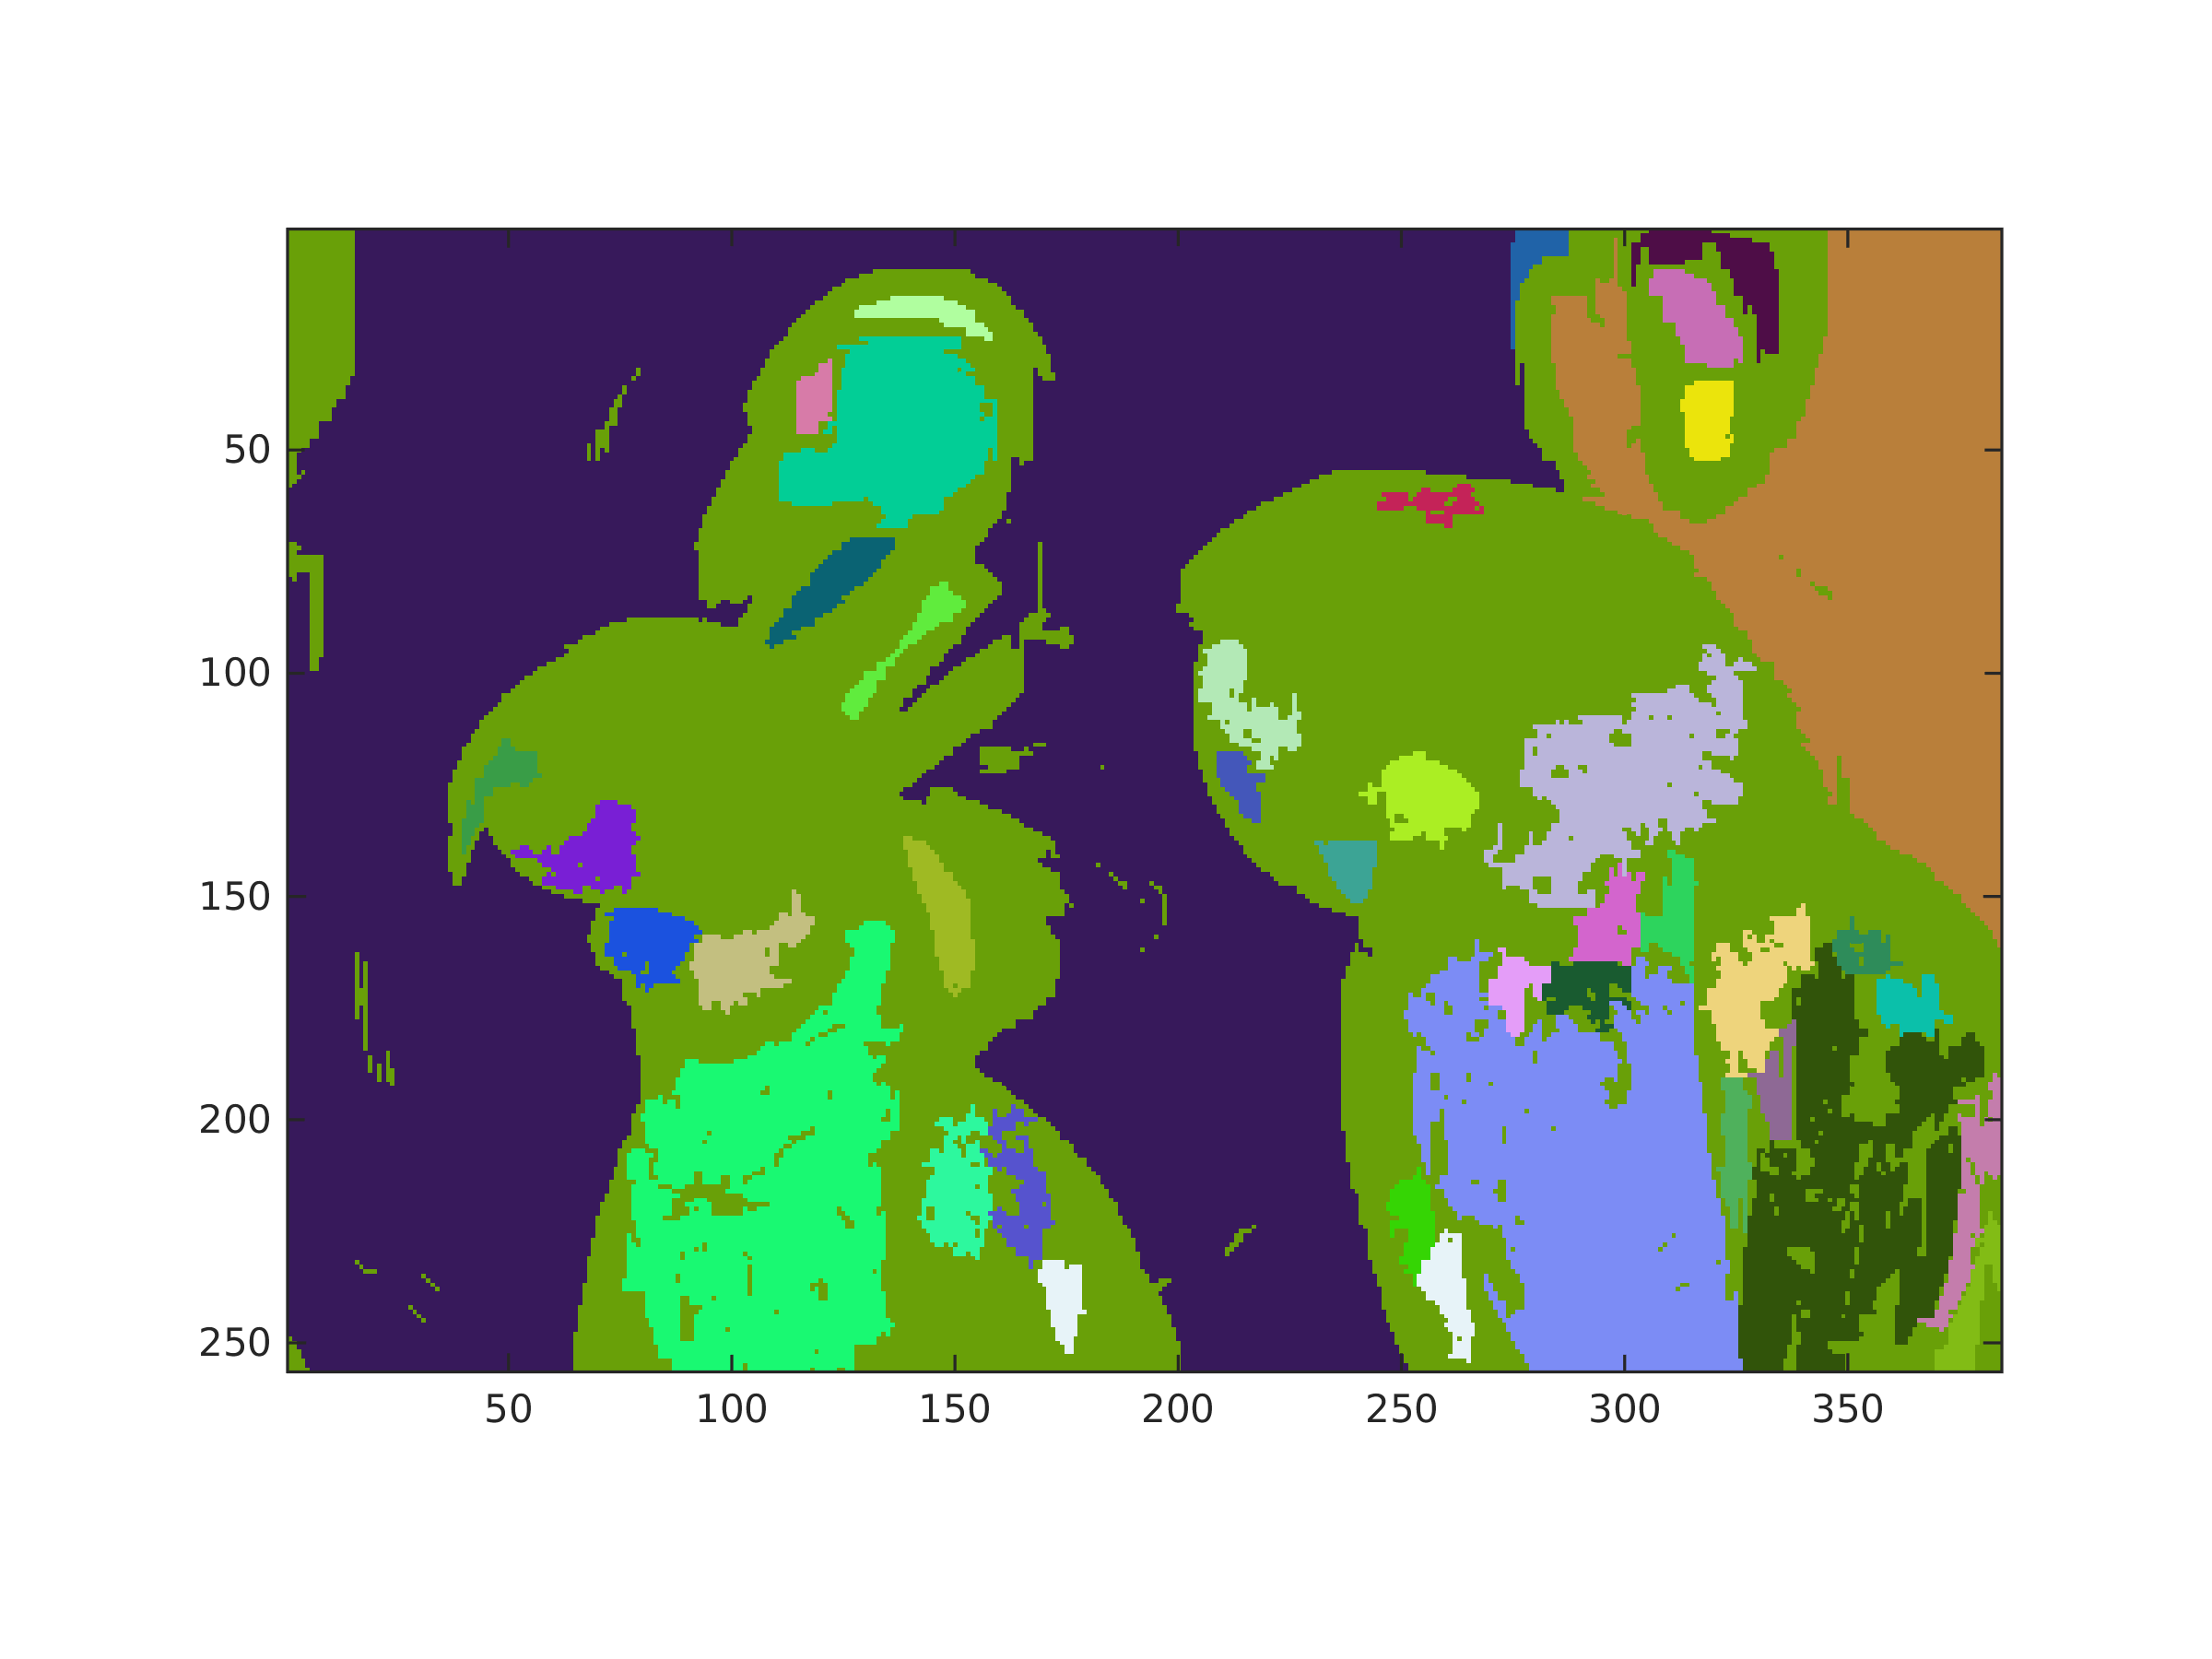
\includegraphics[width=0.65\textwidth]{img22gd2_sm2.png}
			\caption{Randomly colored segmentation for $T=2$}
		\end{center}
	\end{figure}

\subsection{Plot image segmentation for $T=3$}
	\begin{figure}[h]
		\begin{center}
			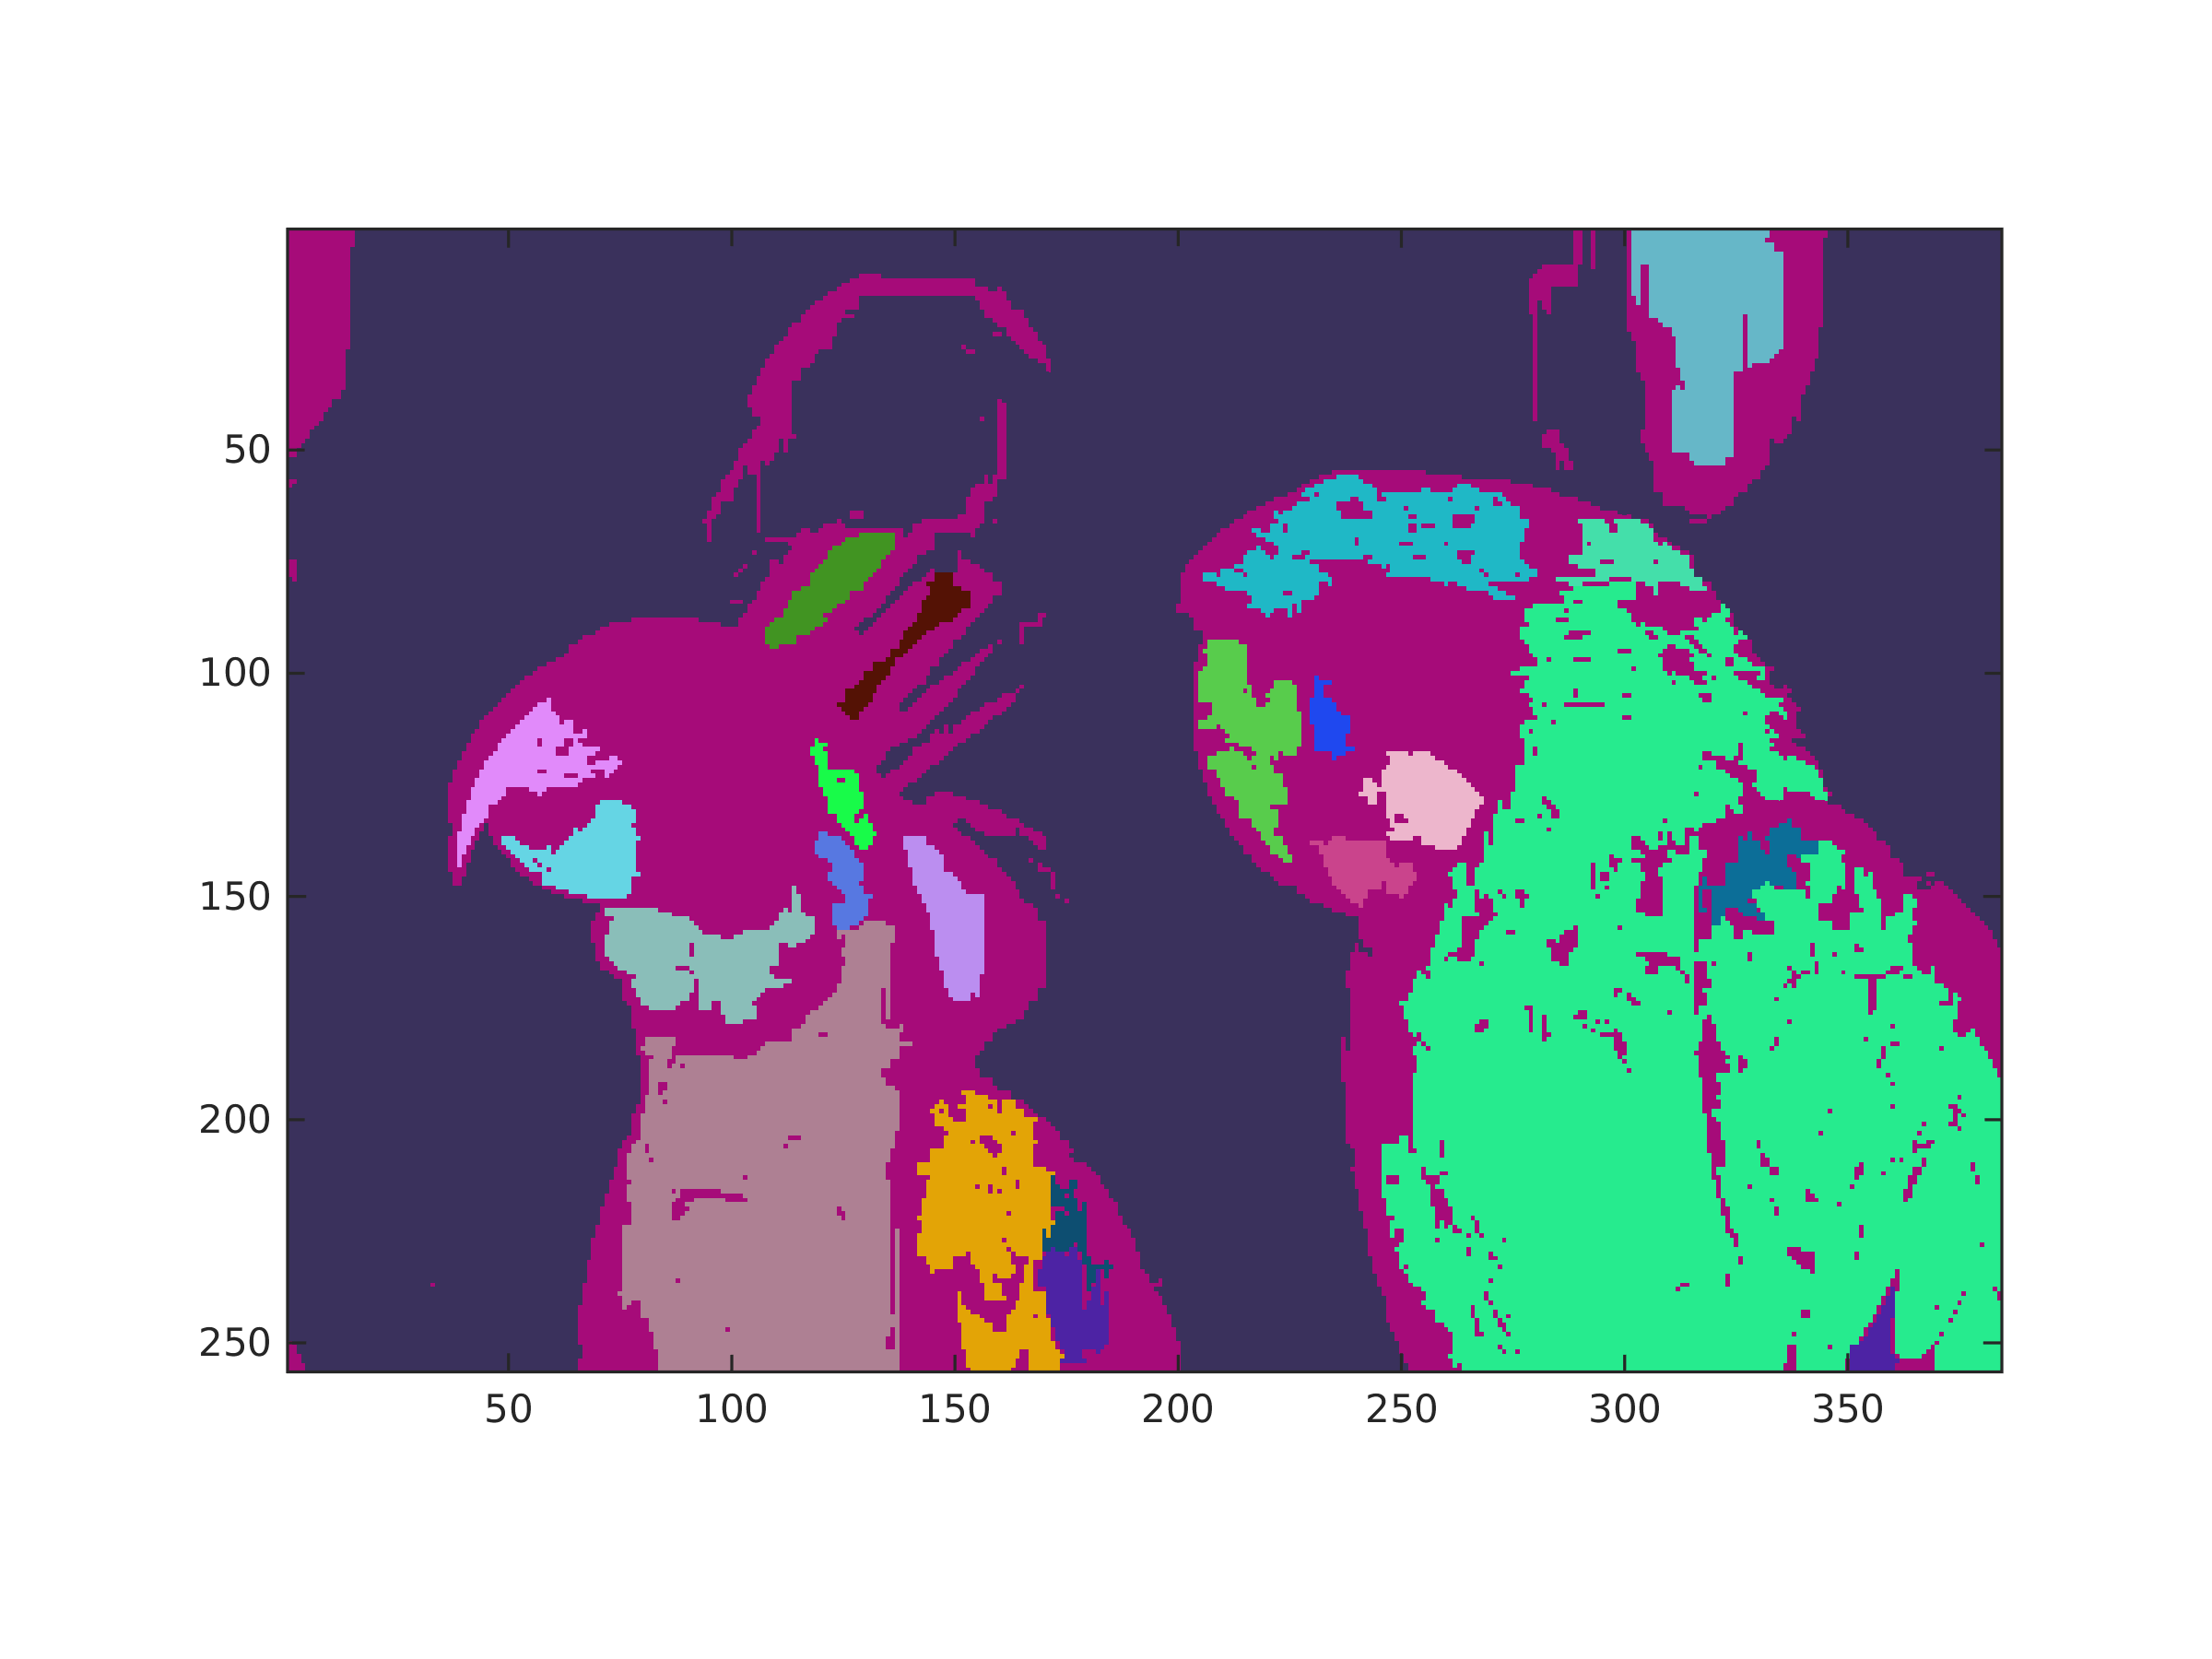
\includegraphics[width=0.65\textwidth]{img22gd2_sm3.png}
			\caption{Randomly colored segmentation for $T=3$}
		\end{center}
	\end{figure}

\subsection{List of the number of regions generated for each threshold}
	\begin{center}
		\begin{tabular}{| l | c |}
		\hline
		& Number of regions \\ \hline
		$T=1$ & 36 \\ \hline
		$T=2$ & 41 \\ \hline
		$T=3$ & 23 \\ \hline
		\end{tabular}
	\end{center}

\subsection{Code listing}
	\subsubsection{segmen.c}
		\inputminted[tabsize=4,breaklines]{c}{segmen.c}

\end{document}
